% Set the stage on AI systems

Within the last half-decade, we have seen an explosion of cloud-based services typically marketed under an \gls{ai} banner. 
Vendors are rapidly pushing out \gls{ai}-based solutions, technologies and products that encapsulate half a century worth of machine-learning research: a \citeyear{LoGiudice:2016wf} report by market research company Forrester captured such growth into four key areas \citep{LoGiudice:2016wf} as replicated in  \cref{fig:introduction:ai-products}. % TODO: Cite all the papers from research products OR mlass. 
Moreover, developers eager to develop a next generation of software are shifting away from mobile-first to `\gls{ai}-first' apps, that will reason, sense, think, act, listen, speak and execute our whims right within the palms of our hands. Most prominently spearheading this wave of \gls{ai}-first thinking is Google, as evident through their 2018 rebranding of \textit{Google Research} to \textit{Google AI} \citep{Howard:2018tz}.

\begin{figure}[thp]
\centering
\caption{A Broad Range of AI-Based Products And Services Is Already Visible. (From \citep{LoGiudice:2016wf}.)}
\label{fig:introduction:ai-products}
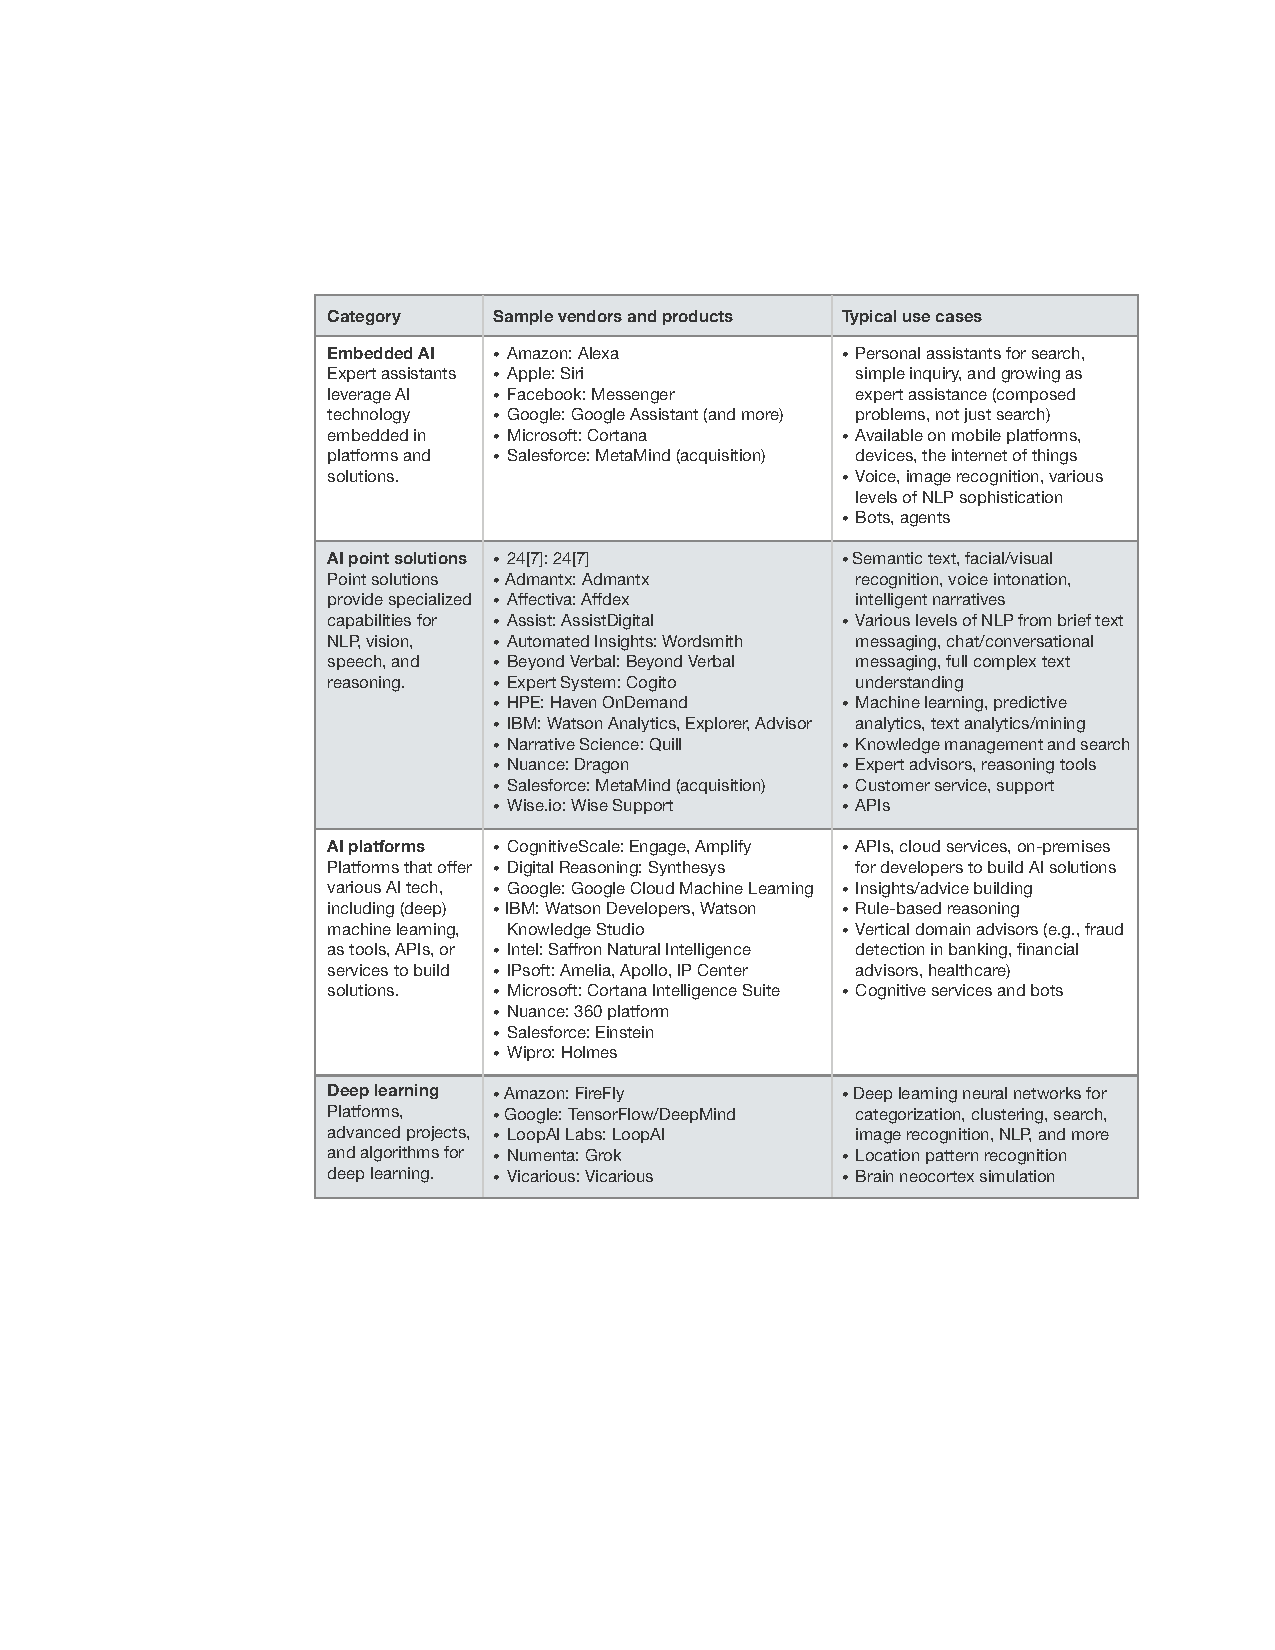
\includegraphics{ai-products}
\end{figure}

These services aim to lower the entry barrier to develop, test and deploy \gls{ai}-first software in both skill and time. 
Software engineers needn't require a formal training in machine-learning nor a strong understanding of mathematics: thus, \textit{skill required} is reduced. The training of such classifiers involves the laborious process of sourcing, curating and labelling large datasets: using such services does not, and thus \textit{time} is reduced. To this end, they needn't require much machine-learning expertise or experience at all; instead, the process is abstracted behind an \gls{api} call, only requiring knowledge on how to use a RESTful architecture \tocite{Restful thesis} to access the cloud service. 

To contrast this with more traditional means, a developer may choose to write up a deep-learning \gls{nn} (for example) and train it using their own dataset. While this is laborious in time and demands significant knowledge in machine learning, the developer has full control over the models she creates. Alternatively, she may choose to download a pre-trained model and \gls{ml} framework, such as Tensorflow \citep{Tensorflow}; less demanding in time but still requiring the knowledge to wire-up models with frameworks.

With less time and skill required to build \gls{AI}-first apps using these cloud services,  these services have begun to gain traction within developer circles: \cref{fig:introduction:stackoverflow-trends} shows the increasing trend of posts since 2014 on StackOverflow that categorise popular computer vision cloud APIs. A growing popularity into such services sparked varied nomenclature: Cognitive Services, Machine Learning as a Service \citep{Ribeiro:2015dz}, Cloud ML and so on. We refer to such services as Cloud Intelligence Services (\glspl{CIS}), and diagramatically express their usage within \cref{fig:introduction:cloud-intelliegnce-service}.

\begin{figure}[t]
\centering
\caption{Number of posts categorised on StackOverflow under popular computer vision cloud intelligence services. Query run on 12 October 2018 using StackExchange Data Explorer. Refer to \url{https://data.stackexchange.com/stackoverflow/query/910188} for full query.}
\label{fig:introduction:stackoverflow-trends}
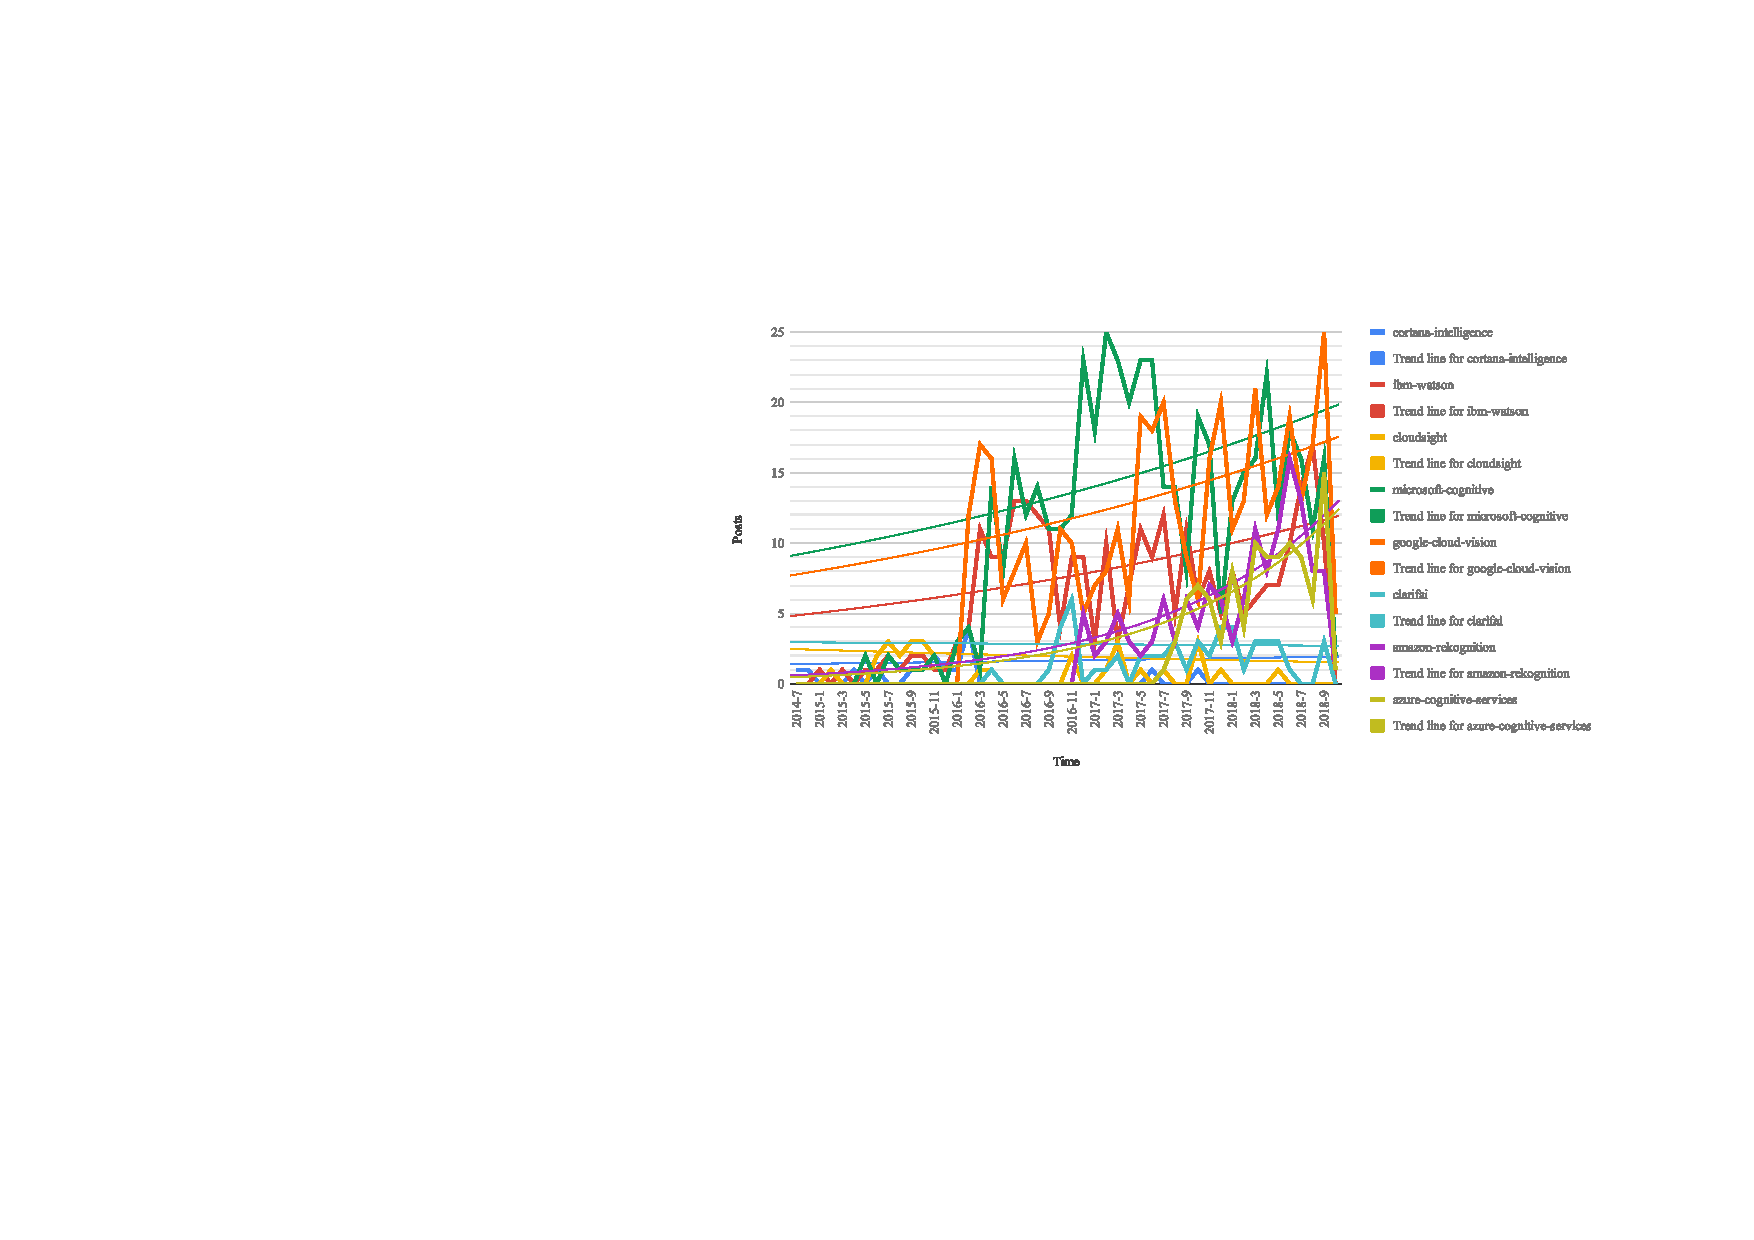
\includegraphics{stackoverflow-trends}
\end{figure}

\begin{figure}[th]
\centering
\caption{Overview of Cloud Intelligence Services.}
\label{fig:introduction:cloud-intelliegnce-service}
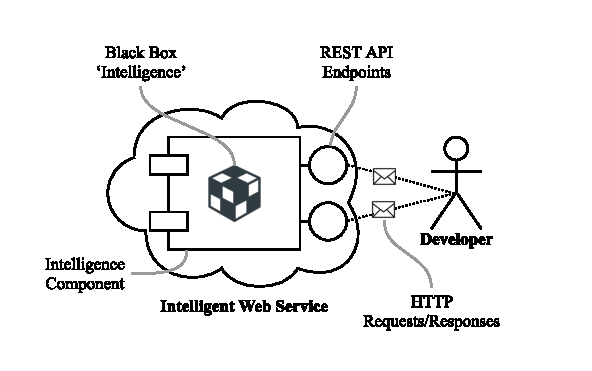
\includegraphics{cloud-intelliegnce-service}
\end{figure}
 
 
A developer accesses a \gls{cis} component via a RESTful API endpoint(s). The input and response communicate through HTTP, typically as JSON content. The `intelligence' component masks intelligence through a black-box. We do not refer to the `intelligence' through the lenses of \textit{artificial} intelligence as the nature of these services may mask human intelligence, as noted by previous work \tocite{Paper Scott told me about about humans tagging}. Their response is hence used by the developer in whichever use case they would like.

While there are many types of \glspl{CIS} evident, we scope the work investigated to \gls{cv} analysers (e.g., \citep{GoogleCloud:Home,Azure:Home,AWS:Home,Pixlab:Home,IBM:Home,Cloudsight:Home,Clarifai:Home,DeepAI:Home,Imagaa:Home,Talkwaler:Home}). The ubiquity of \gls{cv} \glspl{cis} is exemplified through evermore growing applications that use these APIs: aiding the vision-impaired \citep{Reis:2018cp,daMotaSilveira:2017vp}, accounting  \citep{Marshall:2018uj}, data analytics \citep{Iyengar:2017fb}, and student education \citep{Dibia:2017iy}. 
  
  
%  Paper 2:
%* RQ1. How do software engineers evaluate (knowledge representation) machine learning APIs for use in an application?
%   * Motivation: to provide insights into the current practice
%   * Method: Survey
%* RQ2. Do software engineers follow best practices when evaluating machine learning APIs?
%   * Motivation: to compare best practice with actual practice
%   * Survey